\documentclass[11pt,a4paper]{article}

\usepackage[utf8]{inputenc}
\usepackage[margin=1in]{geometry}
\usepackage{amsmath,amssymb,amsfonts}
\usepackage{graphicx}
\usepackage{booktabs}
\usepackage{hyperref}
\usepackage{xcolor}
\usepackage{titlesec}
\usepackage{fancyhdr}
\usepackage{enumitem}
\usepackage{tcolorbox}
\usepackage{tabularx}
\usepackage{tikz}
\usetikzlibrary{shapes.geometric, arrows, positioning, fit, backgrounds}

% Page Geometry & Header setup
\setlength{\headheight}{14pt}
\addtolength{\topmargin}{-2pt}

% Color definitions
\definecolor{primaryblue}{RGB}{24, 76, 120}
\definecolor{secondaryteal}{RGB}{0, 150, 136}
\definecolor{accentorange}{RGB}{238, 76, 44}
\definecolor{darkgray}{RGB}{45, 52, 58}
\definecolor{lightgraybg}{RGB}{245, 247, 250}

% Hyperref setup
\hypersetup{
    colorlinks=true,
    linkcolor=primaryblue,
    filecolor=secondaryteal,
    urlcolor=primaryblue,
    citecolor=accentorange
}

% Header and Footer
\pagestyle{fancy}
\fancyhf{}
\rhead{\textcolor{darkgray}{\small DIP+PINN Satellite Cloud Removal Framework}}
\lhead{\textcolor{darkgray}{\small Technical Reference Report}}
\rfoot{\textcolor{darkgray}{\small Page \thepage}}
\renewcommand{\headrulewidth}{0.4pt}
\renewcommand{\footrulewidth}{0.4pt}

% Section styling
\titleformat{\section}{\Large\bfseries\color{primaryblue}}{\thesection}{1em}{}[\titlerule]
\titleformat{\subsection}{\large\bfseries\color{secondaryteal}}{\thesubsection}{1em}{}
\titleformat{\subsubsection}{\normalsize\bfseries\color{darkgray}}{\thesubsubsection}{1em}{}

\begin{document}

% Title Banner
\begin{titlepage}
    \centering
    \vspace*{1.2cm}
    
    {\Huge \bfseries \color{primaryblue} Physics-Informed Deep Image Prior for Satellite Cloud Removal and Multi-Spectral Restoration\par}
    \vspace{0.8cm}
    {\Large \textbf{Comprehensive Technical Architecture, Physical Formulations, and System Specification}\par}
    
    \vspace{1.2cm}
    
    \begin{tcolorbox}[colback=lightgraybg,colframe=primaryblue,width=0.95\textwidth,arc=3mm]
        \centering
        \textbf{Framework:} Deep Image Prior (DIP) + Physics-Informed Neural Networks (PINN)\\
        \textbf{Backend Engine:} Python 3.10+, PyTorch (CUDA), FastAPI, Rasterio, GDAL\\
        \textbf{Frontend Interface:} HTML5, JavaScript (ES6+), Glassmorphism Dark Theme, Chart.js\\
        \textbf{Datasets:} RICE Benchmark Dataset (RICE-1, RICE-2) \& ESA Copernicus Sentinel-2A
    \end{tcolorbox}
    
    \vspace{1.5cm}
    
    \begin{minipage}{0.9\textwidth}
    \textbf{Executive Summary:}\\
    \small
    This document provides an exhaustive reference report for the satellite cloud removal and explainable AI platform. The system couples the unsupervised inductive bias of Deep Image Prior (DIP) with the physical governing laws of atmospheric radiative transfer equations (PINN). The software provides 13 dedicated operational modules for zero-shot cloud removal, thin haze defogging, dense cloud penetration, and full-scene multispectral Sentinel-2 tile reconstruction.
    \end{minipage}
    
    \vfill
    {\large \textbf{Generated:} \today \par}
\end{titlepage}

\tableofcontents
\newpage

% SECTION 1: ARCHITECTURE
\section{System Architecture \& Operational Flow}

The platform comprises an asynchronous high-performance architecture dividing frontend telemetry, high-throughput REST/WebSocket services, physics-informed optimization solvers, and geospatial raster pipelines.

\subsection{Architectural Flow Diagram}

\begin{center}
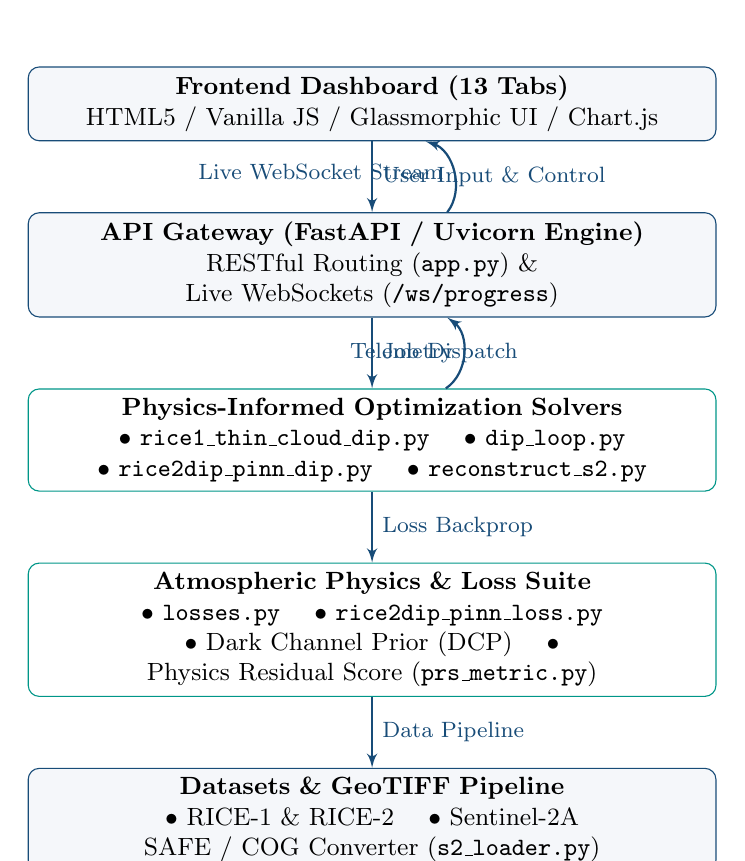
\begin{tikzpicture}[node distance=1.3cm, auto,
    block/.style={rectangle, draw=primaryblue, fill=lightgraybg, text width=8.5cm, text centered, rounded corners, minimum height=0.9cm, font=\small},
    engine/.style={rectangle, draw=secondaryteal, fill=white, text width=8.5cm, text centered, rounded corners, minimum height=0.9cm, font=\small},
    line/.style={draw, -latex', thick, color=primaryblue}]
    
    \node [block] (ui) {\textbf{Frontend Dashboard (13 Tabs)}\\HTML5 / Vanilla JS / Glassmorphic UI / Chart.js};
    \node [block, below=0.9cm of ui] (api) {\textbf{API Gateway (FastAPI / Uvicorn Engine)}\\RESTful Routing (\texttt{app.py}) \& Live WebSockets (\texttt{/ws/progress})};
    \node [engine, below=0.9cm of api] (dl) {\textbf{Physics-Informed Optimization Solvers}\\
    $\bullet$ \texttt{rice1\_thin\_cloud\_dip.py} \quad $\bullet$ \texttt{dip\_loop.py}\\
    $\bullet$ \texttt{rice2dip\_pinn\_dip.py} \quad $\bullet$ \texttt{reconstruct\_s2.py}};
    \node [engine, below=0.9cm of dl] (physics) {\textbf{Atmospheric Physics \& Loss Suite}\\
    $\bullet$ \texttt{losses.py} \quad $\bullet$ \texttt{rice2dip\_pinn\_loss.py}\\
    $\bullet$ Dark Channel Prior (DCP) \quad $\bullet$ Physics Residual Score (\texttt{prs\_metric.py})};
    \node [block, below=0.9cm of physics] (data) {\textbf{Datasets \& GeoTIFF Pipeline}\\
    $\bullet$ RICE-1 \& RICE-2 \quad $\bullet$ Sentinel-2A SAFE / COG Converter (\texttt{s2\_loader.py})};
    
    \path [line] (ui) -- node[right, font=\footnotesize] {User Input \& Control} (api);
    \path [line] (api) -- node[right, font=\footnotesize] {Job Dispatch} (dl);
    \path [line] (dl) -- node[right, font=\footnotesize] {Loss Backprop} (physics);
    \path [line] (physics) -- node[right, font=\footnotesize] {Data Pipeline} (data);
    \path [line] (dl) to[bend right=55] node[left, font=\footnotesize] {Telemetry} (api);
    \path [line] (api) to[bend right=55] node[left, font=\footnotesize] {Live WebSocket Stream} (ui);
\end{tikzpicture}
\end{center}

\newpage
% SECTION 2: MATHEMATICAL FORMULATIONS
\section{Atmospheric Scattering Physics \& Loss Objectives}

\subsection{Koschmieder Radiative Transfer Model}
Degradation in optical remote sensing is modeled via atmospheric radiative transfer:
\begin{equation}
    I(x) = J(x) \cdot t(x) + A(x) \cdot \big(1 - t(x)\big)
\end{equation}
where $I(x)$ is the observed degraded cloudy image, $J(x)$ is the clear surface radiance, $t(x) \in (0, 1]$ is the atmospheric transmission medium map, and $A(x)$ is the airlight radiance vector.

\subsection{Coupled Deep Image Prior (DIP) Generator}
An untrained neural generator network $f_\theta(z)$ with noise code $z \sim \mathcal{N}(0, \sigma^2 I)$ maps directly to surface radiance and medium transmission:
\begin{equation}
    \big(\hat{J}_\theta(z), \hat{t}_\theta(z)\big) = f_\theta(z)
\end{equation}

\subsection{Composite Physics-Informed Loss Objective}
The network parameters $\theta$ are optimized per-image at inference time via:
\begin{equation}
    \mathcal{L}_{\text{total}}(\theta) = \lambda_{\text{rec}} \mathcal{L}_{\text{rec}} + \lambda_{\text{PINN}} \mathcal{L}_{\text{PINN}} + \lambda_{\text{DCP}} \mathcal{L}_{\text{DCP}} + \lambda_{\text{TV}} \mathcal{L}_{\text{TV}} + \lambda_{\text{perc}} \mathcal{L}_{\text{perc}}
\end{equation}

\begin{tcolorbox}[colback=lightgraybg,colframe=secondaryteal,title=\textbf{Mathematical Loss Formulation Summary}]
\begin{enumerate}[leftmargin=*]
    \item \textbf{Radiative Transfer Physics Loss ($\mathcal{L}_{\text{PINN}}$):}
    $$\mathcal{L}_{\text{PINN}} = \frac{1}{|\Omega|} \sum_{x \in \Omega} \left\| I(x) - \left( \hat{J}(x)\hat{t}(x) + A\big(1 - \hat{t}(x)\big) \right) \right\|_2^2$$
    \item \textbf{Dark Channel Prior Regularizer ($\mathcal{L}_{\text{DCP}}$):}
    $$\mathcal{L}_{\text{DCP}}(\hat{J}) = \frac{1}{|\Omega|} \sum_{x \in \Omega} \left( \min_{c \in \{R,G,B\}} \left( \min_{y \in \Omega(x)} \hat{J}^c(y) \right) \right)^2$$
    \item \textbf{Total Variation Regularization ($\mathcal{L}_{\text{TV}}$):}
    $$\mathcal{L}_{\text{TV}}(\hat{J}, \hat{t}) = \|\nabla_x \hat{J}\|_1 + \|\nabla_y \hat{J}\|_1 + \mu \left( \|\nabla_x \hat{t}\|_1 + \|\nabla_y \hat{t}\|_1 \right)$$
    \item \textbf{Perceptual Feature Loss ($\mathcal{L}_{\text{perc}}$):}
    $$\mathcal{L}_{\text{perc}}(\hat{J}, I) = \sum_{l} \frac{1}{C_l H_l W_l} \|\phi_l(\hat{J}) - \phi_l(I)\|_2^2$$
\end{enumerate}
\end{tcolorbox}

\newpage
% SECTION 3: TAB SPECIFICATIONS
\section{Exhaustive Breakdown of Dashboard Tabs}

The frontend web suite is partitioned into 13 dedicated operational views:

\subsection{Tab 1: RICE 1 Explorer (\texttt{tab\_classification.html})}
\begin{itemize}[noitemsep]
    \item \textbf{Backend Files:} \texttt{rice1\_thin\_cloud\_dip.py}, \texttt{rice1\_thin\_cloud\_losses.py}
    \item \textbf{Frontend Script:} \texttt{web/static/rice1\_explorer/rice1\_explorer.js}
    \item \textbf{Goal:} Thin cirrus cloud defogging on 500 paired RICE-1 images.
    \item \textbf{Key Outputs:} Live transmission map $t(x)$ visualization, real-time loss tracking.
\end{itemize}

\subsection{Tab 2: RICE 2 Explorer (\texttt{tab\_rice2\_classification.html})}
\begin{itemize}[noitemsep]
    \item \textbf{Backend Files:} \texttt{dip\_loop.py}, \texttt{losses.py}
    \item \textbf{Frontend Script:} \texttt{web/static/rice2\_explorer/rice2\_explorer.js}
    \item \textbf{Goal:} Thick cloud removal on 450 RICE-2 triplets (cloud, label, binary mask).
    \item \textbf{Key Outputs:} Mask-weighted loss optimization, PSNR/SSIM live telemetry.
\end{itemize}

\subsection{Tab 3: RICE 2 DIP+PINN Explorer (\texttt{tab\_rice2\_page.html})}
\begin{itemize}[noitemsep]
    \item \textbf{Backend Files:} \texttt{rice2dip\_pinn\_dip.py}, \texttt{rice2dip\_pinn\_loss.py}, \texttt{generate\_rice2\_pdf\_report.py}
    \item \textbf{Frontend Script:} \texttt{web/static/rice2\_app.js}
    \item \textbf{Goal:} Coupled neural solver for thick cloud penetration and shadow removal.
    \item \textbf{Key Outputs:} PDF research report export and interactive multi-loss tuning.
\end{itemize}

\subsection{Tab 4: DIP+PINN General Optimization (\texttt{tab\_dippinn.html})}
\begin{itemize}[noitemsep]
    \item \textbf{Backend Files:} \texttt{dip\_loop.py}, \texttt{losses.py}
    \item \textbf{Goal:} Zero-shot unsupervised image restoration on custom user-uploaded imagery.
\end{itemize}

\subsection{Tab 5 \& 6: Cloud Detection (\texttt{tab\_detection.html}) \& Removal (\texttt{tab\_removal.html})}
\begin{itemize}[noitemsep]
    \item \textbf{Backend Files:} \texttt{models/segmentation\_unet.py}, \texttt{inference\_cloud\_removal.py}
    \item \textbf{Goal:} Rapid feedforward cloud mask segmentation and single-pass neural inpainting.
\end{itemize}

\subsection{Tab 7: Sentinel-2A Satellite Workspace (\texttt{tab\_s2\_workspace.html})}
\begin{itemize}[noitemsep]
    \item \textbf{Backend Files:} \texttt{s2\_loader.py}, \texttt{reconstruct\_s2.py}, \texttt{convert\_all\_cogs.py}
    \item \textbf{Frontend Script:} \texttt{web/static/s2\_workspace.js}
    \item \textbf{Products:} China, Vidarbha (Nagpur/Yavatmal), Chandigarh SAFE products.
    \item \textbf{Goal:} True Color RGB, False Color NIR, Agriculture indices, and full-tile inpainting.
\end{itemize}

\subsection{Tab 8--13: Baseline, Evaluation, and Diagnostic Modules}
\begin{itemize}[noitemsep]
    \item \textbf{Tab 8 (Supervised U-Net):} \texttt{tab\_supervised\_unet.html} (Supervised training \& validation logs).
    \item \textbf{Tab 9 (RICE Benchmark):} \texttt{tab\_rice\_bench.html}, \texttt{evaluate.py} (Multi-model benchmark suite).
    \item \textbf{Tab 10 (Metrics Suite):} \texttt{tab\_metrics.html}, \texttt{prs\_metric.py} (Physics Residual Score \& Radar charts).
    \item \textbf{Tab 11 (Hyperparameter Guide):} \texttt{tab\_hyperparameter\_guide.html}, \texttt{configs/} (Preset tuning manual).
    \item \textbf{Tab 12 (Methodology):} \texttt{tab\_methodology.html} (Radiative transfer physics derivations).
    \item \textbf{Tab 13 (System Docs):} \texttt{tab\_system\_docs.html}, \texttt{app.py} (Server hardware and OpenAPI endpoints).
\end{itemize}

\newpage
% SECTION 4: MASTER REFERENCE TABLE
\section{Master Reference Matrix}

\begin{table}[h!]
\centering
\small
\renewcommand{\arraystretch}{1.15}
\begin{tabularx}{\textwidth}{@{}lllX@{}}
\toprule
\textbf{\#} & \textbf{Tab Title} & \textbf{Template File} & \textbf{Core Functionality} \\
\midrule
1 & RICE 1 Explorer & \texttt{tab\_classification.html} & Thin cloud defogging \& $t(x)$ estimation \\
2 & RICE 2 Explorer & \texttt{tab\_rice2\_classification.html} & Thick cloud DIP ablation \& live metrics \\
3 & RICE 2 DIP+PINN & \texttt{tab\_rice2\_page.html} & Coupled PINN solver \& PDF generation \\
4 & DIP+PINN Engine & \texttt{tab\_dippinn.html} & Custom upload zero-shot optimization \\
5 & Cloud Detection & \texttt{tab\_detection.html} & Semantic cloud \& shadow segmentation \\
6 & Cloud Removal & \texttt{tab\_removal.html} & Fast feedforward neural inpainting \\
7 & Sentinel-2A & \texttt{tab\_s2\_workspace.html} & Multi-spectral SAFE \& COG full tiles \\
8 & Supervised U-Net & \texttt{tab\_supervised\_unet.html} & Supervised baseline benchmark \\
9 & RICE Benchmark & \texttt{tab\_rice\_bench.html} & Multi-model metrics radar \& tables \\
10 & Metrics Suite & \texttt{tab\_metrics.html} & Physics Residual Score (PRS) evaluation \\
11 & Hyperparameters & \texttt{tab\_hyperparameter\_guide.html} & Interactive loss parameter handbook \\
12 & Methodology & \texttt{tab\_methodology.html} & Atmospheric radiative transfer physics \\
13 & System Docs & \texttt{tab\_system\_docs.html} & GPU telemetry \& OpenAPI live specs \\
\bottomrule
\end{tabularx}
\caption{System Mapping Matrix across Dashboard Views and Capabilities.}
\end{table}

\section{System Execution Instructions}

\begin{enumerate}
    \item \textbf{Activate Environment \& Install Requirements:}
    \begin{verbatim}
    python -m venv .venv
    .\.venv\Scripts\Activate.ps1
    pip install -r requirements.txt
    \end{verbatim}
    \item \textbf{Run the Application:}
    \begin{verbatim}
    python main.py
    \end{verbatim}
    Open the dashboard in a web browser at \url{http://127.0.0.1:8000}.
\end{enumerate}

\end{document}
